\tikzstyle{input_neuron}=[circle,draw=red!50,fill=red!10,thick,minimum size=6mm]
\tikzstyle{hidden_neuron}=[circle,draw=blue!50,fill=cyan!10,thick,minimum size=6mm]
\tikzstyle{output_neuron}=[circle,draw=green!50,fill=green!10,thick,minimum size=6mm]
\tikzstyle{input}=[circle,draw=black!50,fill=black!20,thick,minimum size=6mm]

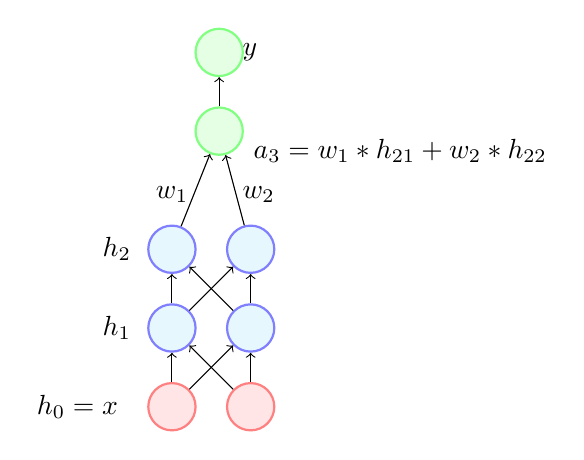
\begin{tikzpicture}
	
	\node [input_neuron] (neuron01) at (7,6.5){} ;
	\node [input_neuron] (neuron02) at (8,6.5){};
	\node[text width=0.005cm] at (6.8,9.2) {$w_1$};
	\node[text width=0.005cm] at (7.9,9.2) {$w_2$};
	%\node[text width=0.005cm] at (7.9,10.25) {$h_3$};
	\node  at (9.9,9.75) {$a_3 = w_1*h_{21} + w_2 * h_{22}$};
	\node[text width=0.005cm] at (7.9,11.0) {$y$};
	%\node at (9.9,11.5) {$a_3 = w_1*h_{21} + w_2 * h_{22})$};
	
	
	\node (hidden1) at (5.8,6.5){$h_0=x$};
	\node (hidden2) at (6.3,7.5){$h_1$};
	\node (hidden3) at (6.3,8.5){$h_2$};
	%\node(input0) at(7.6,5.8){$h_o = x$};
	%\node(text) at (10,9.3){All outputs are between [0,1]};
	\node [hidden_neuron] (neuron11) at (7,7.5){}  ;
	\node [hidden_neuron] (neuron12) at (8,7.5) {} ;
	%\node [hidden_neuron] (neuron13) at (9,7.5)  ;
	
	\node [hidden_neuron] (neuron21) at (7,8.5){}  ;
	\node [hidden_neuron] (neuron22) at (8,8.5) {} ;
	%\node [hidden_neuron] (neuron23) at (9,8.5)  ;
	
	\node [output_neuron] (neuron42) at (7.6,10.0) {} ;
	\node [output_neuron] (neuron52) at (7.6,11.0) {} ;
	%\draw[->,red](text)--(neuron02);
	%\draw[->,red](text)--(neuron12);
	%\draw[->,red](text)--(neuron22);
	
	\draw[->](neuron01)--(neuron11);
	\draw[->](neuron01)--(neuron12);
	%\draw[->](neuron01)--(neuron13);
	
	\draw[->](neuron02)--(neuron11);
	\draw[->](neuron02)--(neuron12);
	%\draw[->](neuron02)--(neuron13);
	
	%\draw[->](neuron03)--(neuron11);
	%\draw[->](neuron03)--(neuron12);
	%\draw[->](neuron03)--(neuron13);
	
	\draw[->](neuron11)--(neuron21);
	\draw[->](neuron12)--(neuron21);
	%\draw[->](neuron13)--(neuron21);
	
	\draw[->](neuron11)--(neuron22);
	\draw[->](neuron12)--(neuron22);
	%\draw[->](neuron13)--(neuron22);
	
	%\draw[->](neuron11)--(neuron23);
	%\draw[->](neuron12)--(neuron23);
	%\draw[->](neuron13)--(neuron23);
	
	\draw[->](neuron21)--(neuron42);
	\draw[->](neuron22)--(neuron42);
	%\draw[->](neuron23)--(neuron42);
	\draw[->](neuron42)--(neuron52);
	%\node (output1) at (8,10.5){};
	%\node (output0) at (7,10.5){$y_1$};
	
	%\node (output2) at (9,10.5){$y_3$};
	
\end{tikzpicture}